%=====================================================================
\section{Generalization and depth of the learned residual (RQ1, stage 2)}\label{sec:depth}
%=====================================================================
The first RQ1 results (Sections~\ref{sec:koopman} to~\ref{sec:mpc}) left four questions open: does the residual survive a change of plant if it keeps learning, does it help during the capture transients, how sensitive is the result to the MPC settings and to the modelling choices, and does it survive a more realistic truth plant? This section answers them with experiments E8c to E8g. Each was pre-registered in its script, all numbers are from the tables named below, and the places where a first attempt was changed are listed in Section~\ref{sec:budget-dev}.

\subsection{Online adaptation of the residual (E8c)}\label{sec:adaptive}
\begin{plain}
The residual is a fixed correction learned on one plant. Recursive least squares (RLS) keeps adjusting its weights while the drone flies, using each new measurement to correct the last prediction, so that the correction can follow a plant it was not trained on.
\end{plain}
\paragraph{Method.} The 91-function dictionary and its standardization are kept; the $91\times7$ weight matrix is adapted by RLS with one shared covariance (initial value $I$), forgetting factor 0.995 (a memory of about 1\,s) with 0.999 as a sensitivity case, and the output clipped as before (a variant with twice the clip is also reported). The update is causal: at step $k$ it uses the features of step $k-1$ and the measured error $x_k-\hat x^{\text{nom}}_k$, and only afterwards is the residual for step $k$ evaluated (\texttt{AdaptiveResidual}; tested against an explicit RLS step). The covariance trace is bounded (rescaled above ten times its initial value) so that it cannot wind up when the drone sits near the trim and the data carry no new information.

\paragraph{Prediction.} With adaptation running along each test episode, the error on the held-out family B drops to about half of the offline residual's at every horizon (5\,ms: 0.168 against 0.309; 100\,ms: 2.78 against 5.93; 0.5\,s: 8.42 against 17.57), and beats the analytical model up to 200\,ms (5.57 against 7.54 at 200\,ms), but is worse than it from 0.5\,s on (8.42 against 5.13). On the training family A it gives no gain: equal to the offline residual up to 20\,ms and worse beyond (0.5\,s: 1.30 against 0.30), because the adapted weights drift away from a fit that was already right (\texttt{results/tables/e8c\_adaptive\_residual.md}, Part a).

\paragraph{Closed loop.} In the altitude test of E7 the adaptive residual MPC repairs the one plant on which the offline residual was worse than the LQR: on B without thrust loss the steady error is $+0.084$\,m (offline residual $+0.164$, LQR $+0.112$). It matches the offline residual on plant A ($-0.194$ against $-0.193$\,m) and is worse than it on the other A-derived plants (for example $-0.112$ against $-0.066$ on A without thrust loss) and the offset-free controllers and the LQR with an integrator of Section~\ref{sec:offsetfree} remain the better bias remedies. The three adaptive variants differ by at most 0.005\,m on every plant. Combined with the state-model offset-free MPC the bias is 0.000\,m on all six plants, with or without the residual. Capture after a delay on plant A: the adaptive MPC is SAFE for 0 and 10\,ms, like the LQR and better than the offline residual (SAFE at 0\,ms only); at larger delays all fail and the height loss is between the LQR's and the offline residual's.

\paragraph{Adaptation diagnostics.} The covariance guard is active: the trace sits at its cap of 910 and the covariance was rescaled about 1075 times per 8\,s run with $\lambda = 0.995$ (never, with maximum trace 320 to 339, for $\lambda=0.999$): near the trim the data do not excite most of the 91 weights, so their covariance grows until the bound. The covariance matrix stayed positive definite in every run (checked every 50 updates), the clip was active in 1.9\% (A) and 0.7\% (B without thrust loss) of the calls, and the median CVXPY time per step was 5.2 to 6.8\,ms, unchanged by the adaptation. \emph{Limitation:} the adaptation runs in closed loop, so the regressors are correlated with the estimation error (closed-loop identification bias); we did not correct for it.

\begin{figure}[h]
\centering
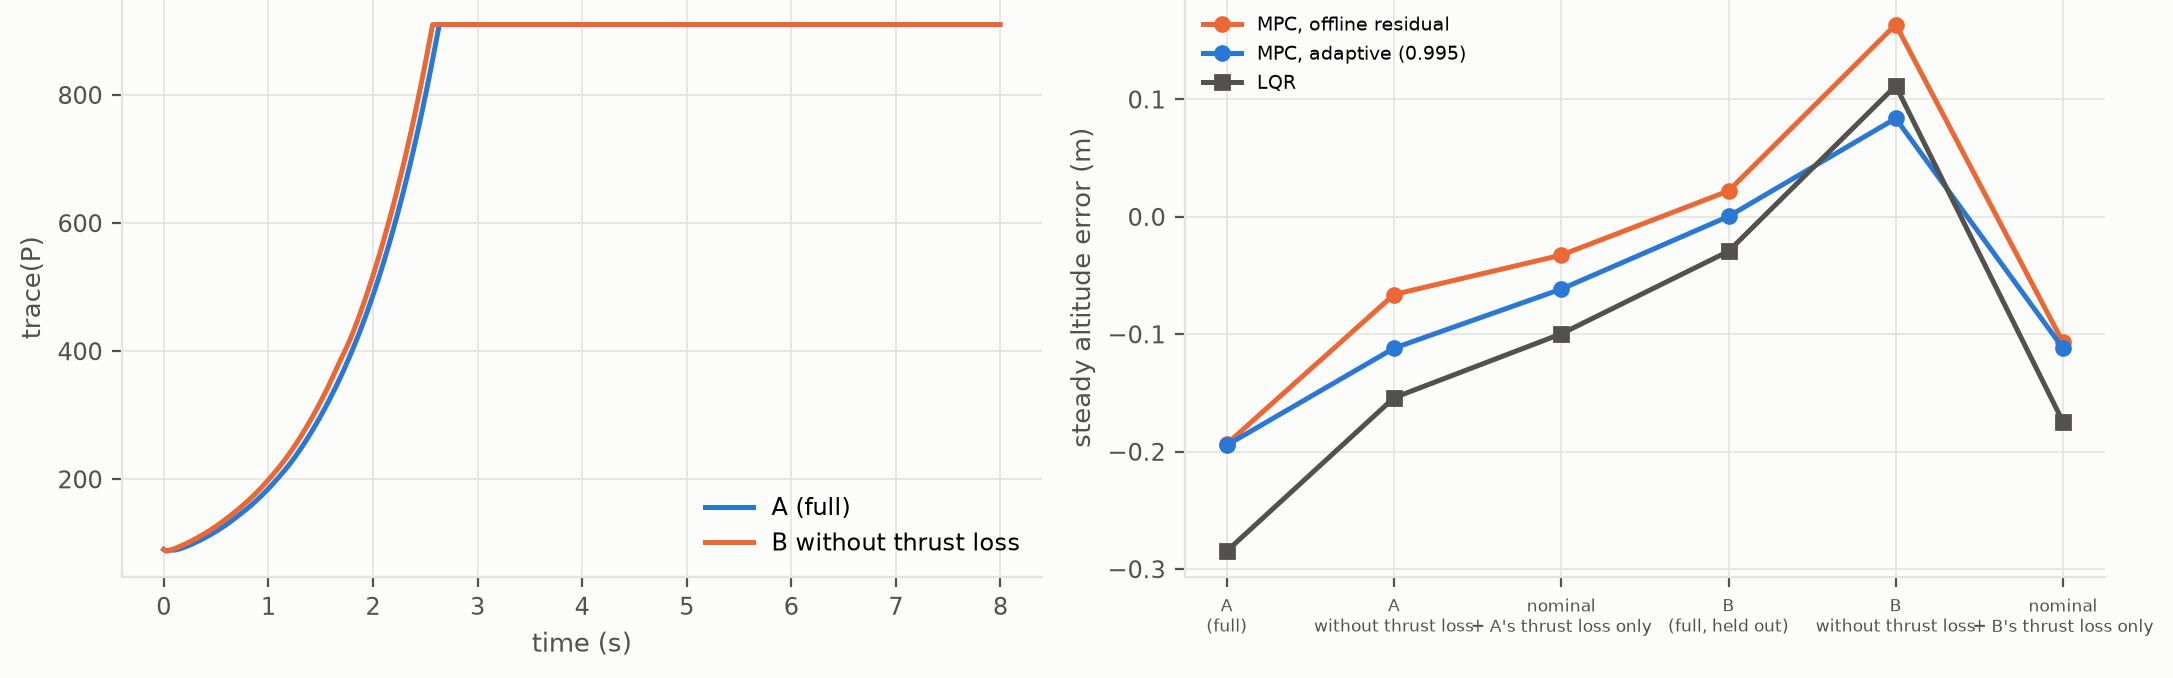
\includegraphics[width=\linewidth]{figures/e8c_adaptive.png}
\caption{E8c. Left: covariance trace of the adaptive residual ($\lambda = 0.995$) on two plants (the cap is 910). Right: steady altitude error by plant for the LQR, the offline residual MPC and the adaptive residual MPC.}\label{fig:e8c}
\end{figure}

\subsection{A residual trained on spin-up transients (E8d)}\label{sec:transient}
The residual of Section~\ref{sec:koopman} was trained near the relaxed hover, but the capture starts far from it (Section~\ref{sec:budget}). We generated capture transients on family A: failures with a random delay $\tau\in[0,20]$\,ms, random pre-failure states, the spin-up at 2.95\,N, and the failure LQR with random excitation after the hand-over, recorded for 4\,s from the hand-over (40 episodes, 32\,000 samples), and trained the residual on the near-trim data plus these, on the transients alone, and with row-normalized regression; test sets are 10 near-trim and 10 new transient episodes. (A first version of the experiment discarded most episodes by a rule that did not fit the data; see Section~\ref{sec:budget-dev}.)

On the held-out transients the near-trim residual is no better than the analytical model (100\,ms: 8.20 against 10.04), as expected from data far outside its training range, while the residual trained with the transients predicts them an order of magnitude better (0.67 for near-trim plus transients and 0.57 for transients alone at 100\,ms; 1.9 and 1.6 at 1\,s). Near the trim, adding the transients costs accuracy at short horizons (100\,ms: 0.214 against 0.116) and helps at long ones (2\,s: 0.71 against 2.55); row normalization did not help. In \emph{closed loop}, however, the better predictor is the worse controller: with the near-trim-plus-transient residual the MPC fails the capture even at $\tau=0$ (height loss 1.97\,m, minimum $n_z=-0.27$, against 0.58\,m and 0.20 for the near-trim residual), and the loss at larger delays is several times larger (30\,ms: 196\,m against 19.5\,m). We did not diagnose why; a plausible reading, not tested, is that a residual that is large and state-dependent during the transient acts as a measured disturbance that the MPC, which holds it constant over the horizon, cannot use consistently. The positive result is that the prediction error far from the hover can be reduced by training on transients; the negative result is that this does not carry over to the capture performance of the MPC as built.

\begin{figure}[h]
\centering
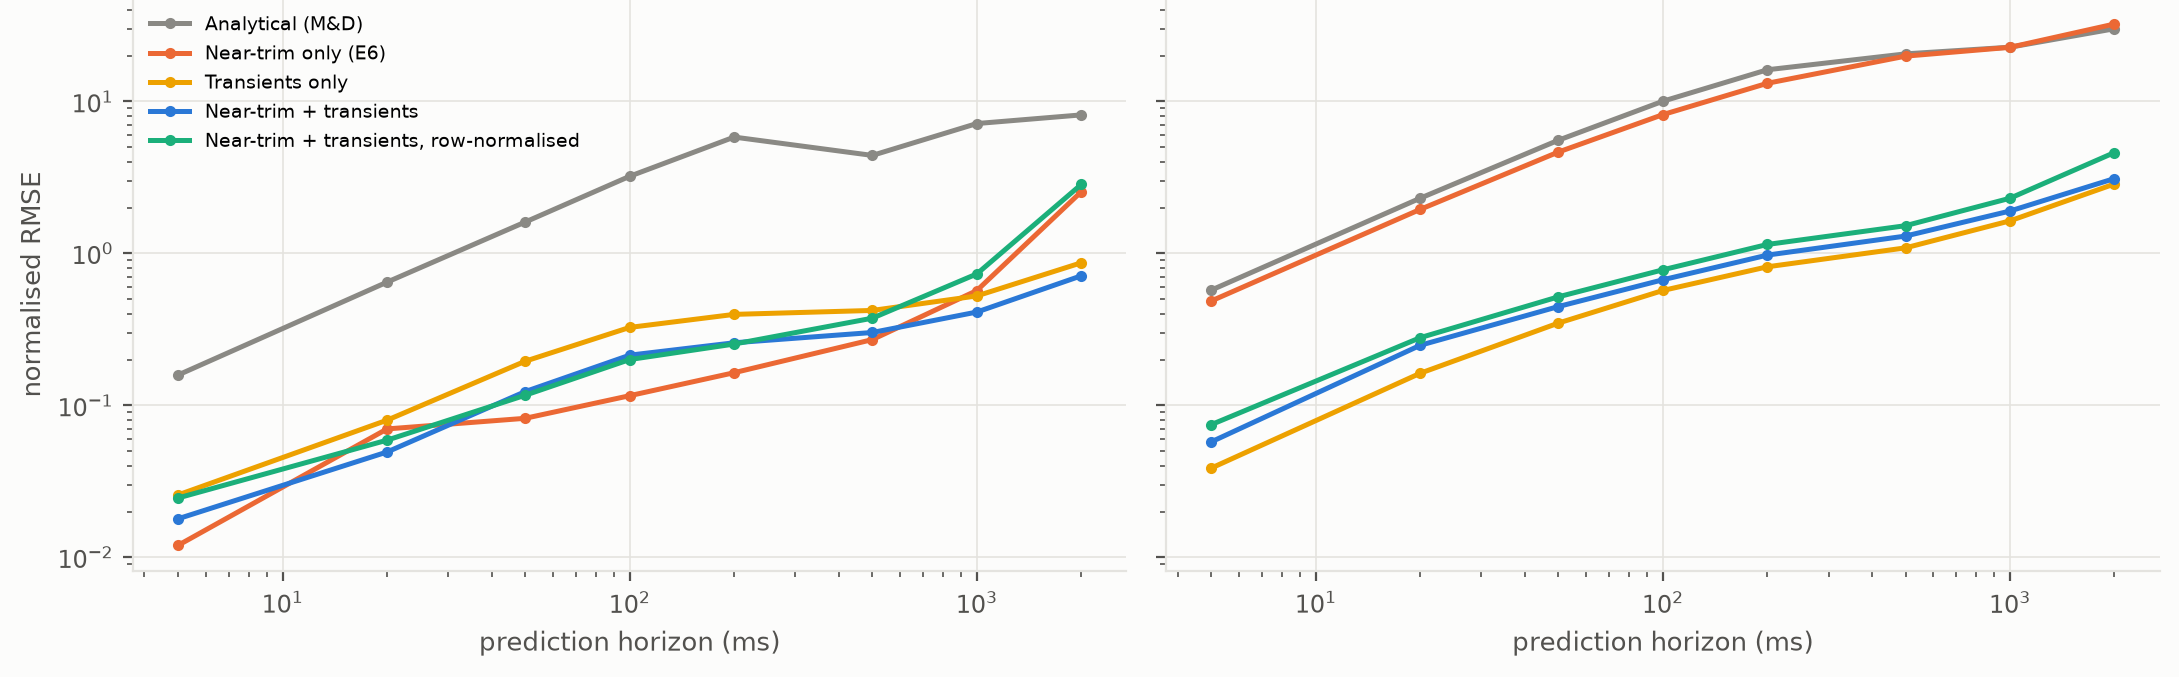
\includegraphics[width=\linewidth]{figures/e8d_spinup.png}
\caption{E8d. Multi-step prediction error of the residual models on held-out near-trim episodes (left) and held-out capture transients (right).}\label{fig:e8d}
\end{figure}

\subsection{Air-relative thrust and quadratic drag in the truth plant (E8g)}\label{sec:realistic}
Our truth plants of Section~\ref{sec:koopman} contain thrust loss, inertia errors and slower motors, but not two effects of the IJRR model that we had validated in \texttt{validation.py}: thrust computed from the propeller speed relative to the air, and quadratic drag. We added them as optional fields of the vehicle parameters (off by default; a test checks that the default dynamics are bit-identical to the previous ones for the nominal plant and for families A and B, and that with the effects on the derivative equals the independent implementation and the published hover rates agree within 1\%) and defined families A$^+$ and B$^+$. Models trained on 40 episodes of A$^+$ predict A$^+$ as before (100\,ms: 0.199 for the full-state EDMDc, 0.180 for the residual) and both fail on B$^+$ (5.98 and 5.87; analytical 3.34), as on A and B; the residual trained on A is much worse than the one trained on A$^+$ on A$^+$ (0.91 against 0.18). In the altitude test the LQR has a larger bias on A$^+$ ($-0.412$\,m against $-0.285$), the residual MPC still reduces it ($-0.273$), the offset-free MPC removes it on all five plants (0.000\,m), the LQR with an integrator leaves at most 0.018\,m, and the residual MPC is again worse than the LQR on the plant without thrust loss (B$^+$: $+0.102$ against $+0.009$\,m). The conclusions of Sections~\ref{sec:mpc} and \ref{sec:offsetfree} therefore survive the more realistic plants (\texttt{results/tables/e8g\_realistic\_plant.md}).

\begin{figure}[h]
\centering
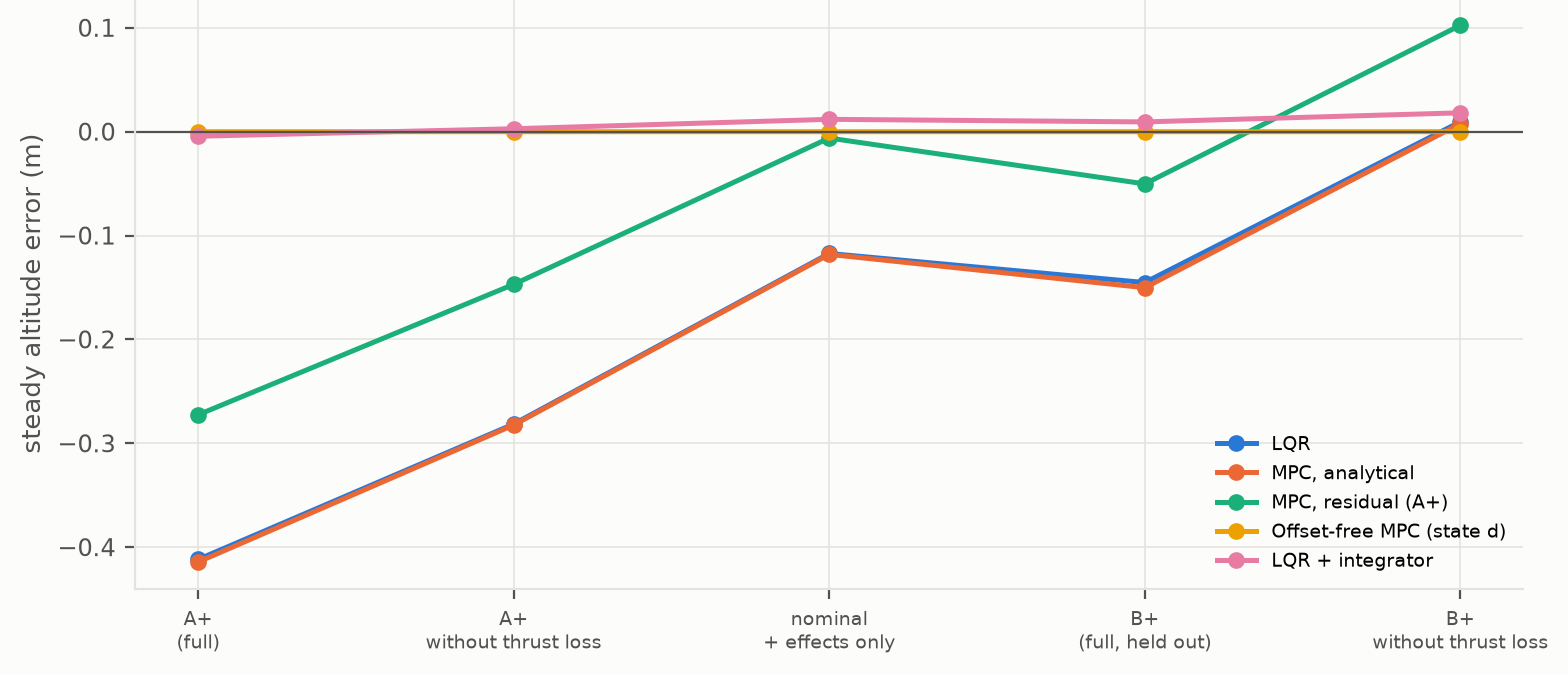
\includegraphics[width=0.8\linewidth]{figures/e8g_plants.png}
\caption{E8g. Steady altitude error by plant and controller on the plants with air-relative thrust and quadratic drag.}\label{fig:e8g}
\end{figure}
